% !TeX TXS-program:compile = txs:///lualatex

\documentclass[a4paper,11pt]{article}
\usepackage[revgoku]{cp-base}
\graphicspath{{./graphics/}}
%variables
\donnees[%
	classe={1\up{ère} 2M2},matiere={[SPÉ.MATHS]},mois=Novembre,annee=2021,typedoc=CHAP,numdoc=4]

%formatage
\author{Pierquet}
\title{\nomfichier}
\hypersetup{pdfauthor={Pierquet},pdftitle={\nomfichier},allbordercolors=white,pdfborder=0 0 0,pdfstartview=FitH}
%fancy
\lhead{\entete{\matiere}}
\chead{\entete{\lycee}}
\rhead{\entete{\classe{} - \mois{} \annee}}
%\rhead{\entete{\classe{} - Chapitre }}
\lfoot{\pied{\matiere}}
\cfoot{\logolycee{}}
\rfoot{\pied{\numeropagetot}}

\begin{document}

\pagestyle{fancy}

\part{CH04 - Second degré, études de signes - Exercices}

\smallskip

\exonum{0}
%
\begin{enumerate}
	\item Étudier le signe des expressions suivantes :
	\begin{enumerate}
		\item $4x^2-7x-3$ ;
		\item $-7x^2+12x-6$ ;
		\item $4x^2-2,4x+0,36$.
	\end{enumerate}
	\item Résoudre les inéquations suivantes :
	\begin{enumerate}
		\item $-x^2+5x+7 \pg 0$ ;
		\item $11x^2+16x-9<10x+8$.
	\end{enumerate}
\end{enumerate}

\medskip

\exonum{2}

\medskip

Résoudre les inéquations suivantes :
%
\begin{enumerate}
	\item $(x-1)(x^2-5x+6)>0$ ;
	\item $\dfrac{-x^2+5x-7}{2x+5} \pp 0$ ;
	\item $x^3-x^2+4x \pg 0$ ;
	\item $\dfrac{3x}{x+1} \pg 5x$.
\end{enumerate}

\medskip

\exonum{2}

\medskip

Résoudre les inéquations suivantes :
%
\begin{enumerate}
	\item $\dfrac{x^2-10x+25}{-5x^2-3x+8} \pp 0$ ;
	\item $\dfrac{-2x}{x+2} \pp \dfrac{3x+2}{x-1}$ ;
	\item $(-x^2+5x-6)(-3x^2+5x-2) \pg 0$.
\end{enumerate}

\medskip

\exonum{3}

\medskip

On considère les fonctions $f$ et $g$ définies par $f(x)=\dfrac{x-1}{x+3}$ et $g(x)=-x-5$.
%
\begin{enumerate}
	\item 
	\begin{enumerate}
		\item Sur la calculatrice, tracer les deux courbes $\mathcallig{C}_f$ et $\mathcallig{C}_g$, avec \ccalg{Xmin=-10}, \ccalg{Xmax=1}, \ccalg{Ymin=-8} et \ccalg{Ymax=8}.%\vspace{-0.2cm}
		\begin{center}
			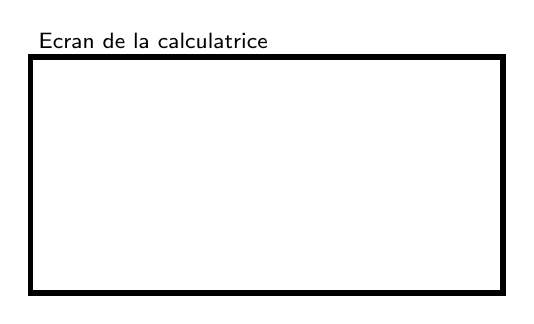
\begin{tikzpicture}[line width=2pt]
				\draw (0,3) node[inner sep=2pt,above right,font=\footnotesize\sffamily] {Ecran de la calculatrice} ;
				\draw (0,0) rectangle (6,3) ;
			\end{tikzpicture}%
		\end{center}%\vspace{-0.2cm}
		\item À l'aide des outils \ccalg{graphiques}, déterminer les coordonnées des points d'intersection de $\mathcallig{C}_f$ et $\mathcallig{C}_g$.
		\item Déterminer la position relative des deux courbes $\mathcallig{C}_f$ et $\mathcallig{C}_g$.
		
		NB : on pourra présenter sous la forme \og Sur l'intervalle \ldots\ldots, $\mathcallig{C}_f$ est \ldots\ldots\ldots\ldots{} de $\mathcallig{C}_g$ \fg.
	\end{enumerate}
	\item Étudier, grâce au signe de $f(x)-g(x)$, la position relative de $\mathcallig{C}_f$ et $\mathcallig{C}_g$.
\end{enumerate}



\end{document}